\let\negmedspace\undefined
\let\negthickspace\undefined
\documentclass[journal]{IEEEtran}
\usepackage[a5paper, margin=10mm, onecolumn]{geometry}
%\usepackage{lmodern} % Uncomment if needed for pdflatex
\usepackage{tfrupee} % Include tfrupee package

\setlength{\headheight}{1cm} % Set the height of the header box
\setlength{\headsep}{0mm}     % Set the distance between the header box and the top of the text

\usepackage{gvv-book}
\usepackage{gvv}
\usepackage{cite}
\usepackage{amsmath,amssymb,amsfonts,amsthm}
\usepackage{algorithmic}
\usepackage{graphicx}
\usepackage{textcomp}
\usepackage{xcolor}
\usepackage{txfonts}
\usepackage{listings}
\usepackage{enumitem}
\usepackage{mathtools}
\usepackage{gensymb}
\usepackage{comment}
\usepackage[breaklinks=true]{hyperref}
\usepackage{tkz-euclide} 
\usepackage{listings}
%\usepackage{gvv}                                        
\def\inputGnumericTable{}                                 
\usepackage[latin1]{inputenc}                                
\usepackage{color}                                            
\usepackage{array}                                            
\usepackage{longtable}                                       
\usepackage{calc}                                             
\usepackage{multirow}                                         
\usepackage{hhline}                                           
\usepackage{ifthen}                                           
\usepackage{lscape}
\usepackage{tikz}
\usepackage{circuitikz}
\usepackage{standalone} % For including external TikZ files

\begin{document}

\bibliographystyle{IEEEtran}
\vspace{3cm}

\title{8.1.3}
\author{EE24BTECH11066 - YERRA AKHILESH}
% \maketitle
% \newpage
% \bigskip
{\let\newpage\relax\maketitle}

\renewcommand{\thefigure}{\theenumi}
\renewcommand{\thetable}{\theenumi}
\setlength{\intextsep}{10pt} % Space between text and floats

\numberwithin{equation}{enumi}
\numberwithin{figure}{enumi}
\renewcommand{\thetable}{\theenumi}
\textbf{Question}:\\
Find the area of the region bounded by $x^2 = 4y, y = 2, y = 4$ and the y-axis in the first quadrant.\\
\textbf{Solution: }\\
\textbf{Theoritical Solution:}\\
Express $x$ in terms of $y$,
\begin{align}
    x = 2 \sqrt{y}\\
    (or) \\
    x = -2 \sqrt{y}
\end{align}
But we should take first equation as we have to find the area in the first quadrant,\\
Area under the curve is given by,
\begin{align}
    A = \int_{2}^{4} 2 \sqrt{y} \, dy\\
    A = 2 \brak{\frac{y^{\frac{3}{2}}}{\frac{3}{2}}} \Big|_2^4\\
    A = \frac{4}{3} \brak{4^{\frac{3}{2}} - 2^{\frac{3}{2}}}\\
    A = \frac{4}{3} \brak{8 - 2\sqrt{2}}\\
    A = 6.895
\end{align}
\textbf{Computational Solution:} Trapezoidal method\\
The difference equation for any general integral is as follows
\begin{align}    
\int_a^b f(x) \, dx \approx \frac{h}{2} \left[ f(x_0) + 2 \sum_{i=1}^{n-1} f(x_i) + f(x_n) \right]   
\end{align}
For n=1000,
\begin{align}    
\int\limits_2^4 f(y) \, dy \approx \frac{h}{2} \left[ (2\sqrt{y_0}) + 2 \sum_{i=1}^{999} (2\sqrt{y_i}) + (2\sqrt{y_{1000})} \right]   
\end{align}
'y' varies from 2 to 4 and x varies accordingly.\\
The code sums up the required values iteratively for 'n'(say 1000) intervals\\
By computing it iteratively(computationally) we get area as 6.895 sq. units \\
Hence, the area we calculated theoretically is verified\\
\begin{figure}[ht!]
   \centering
   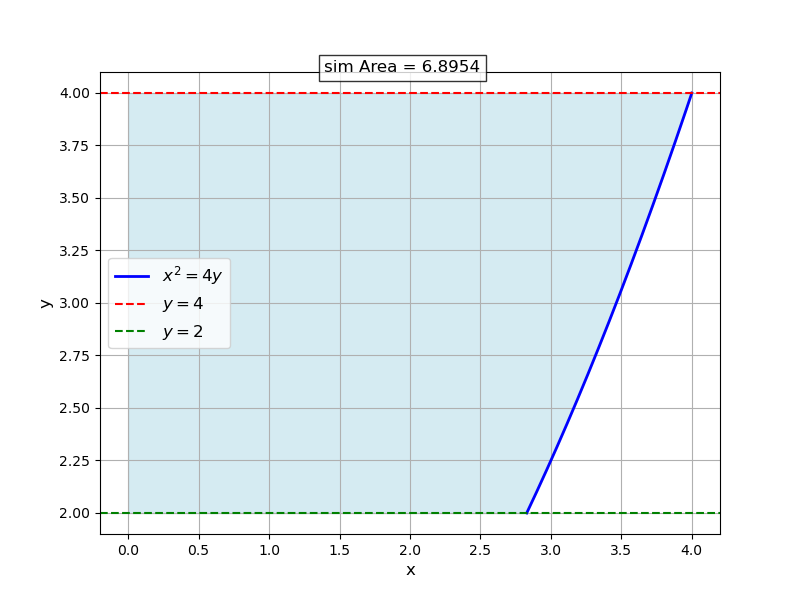
\includegraphics[width=\columnwidth]{figs/Figure_1.png}
\end{figure}
\end{document}
